\section{Building Android Applications with Obfuscation}
\begin{obeylines}
The first step in finding obfuscation fingerprints was to look at the differences between an unobfuscated Android application and an obfuscated Android application. To make this comparison easier to achieve, a simple Android application was written. Each time the Android application was compiled and built, a different obfuscator was used. After all of the applications were obfuscated, each application was disassembled and compared against the unobfuscated disassembly.
\subsection{Simple Android Application}
The Android application that was written included four parts: the main activity, string encryption activity, Fibonacci calculator activity, and get web page activity. Each of the activities attempted to achieve some functionality that could be found in many Android applications. This would result in seeing obfuscation that could be used to identify their correlating fingerprints. Each activity also included extraneous and unused variables and classes that would be affected by each of the obfuscators. The source code for this application is located in Appendix \ref{app:customapp}.
\subsubsection{Main Activity}
The main activity included three input entry boxes with accompanying send buttons. Input was entered, the \emph{Send} button was pushed, and the corresponding activity was called and executed. The main activity can be seen in Figure \ref{fig:mainactivity}. The Java code for this activity is located in Appendix \ref{app:camainactivity} while the activity XML is located in Appendix \ref{app:camainxml}.
\begin{figure}[!ht]
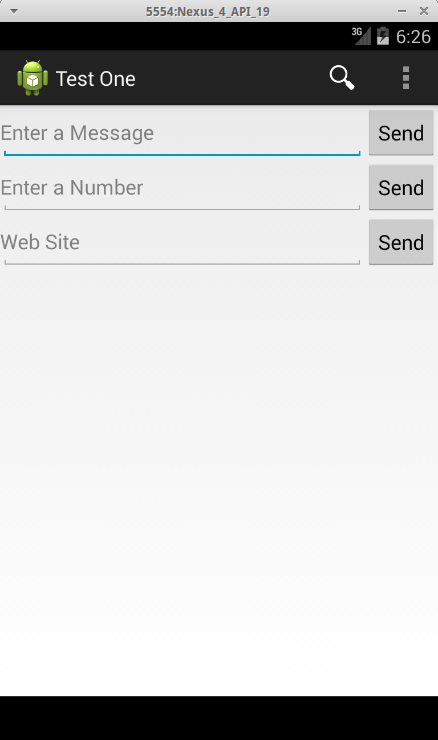
\includegraphics[scale=0.25]{main-activity.png}
\caption{Main Activity Screenshot.\label{fig:mainactivity}}
\end{figure}
\subsubsection{String Encryption Activity}
The string encryption activity used the text entered into the main activity and encrypted it. It would then display the encrypted text in a new activity window. The string activity can be seen in Figure \ref{fig:stringactivity}. The Java code for the string encryption is located in Appendix \ref{app:camessageactivity} and the encryption code is located in Appendix \ref{app:casimplecrypto} and the activity XML is located in Appendix \ref{app:camessagexml}.
\begin{figure}[!ht]
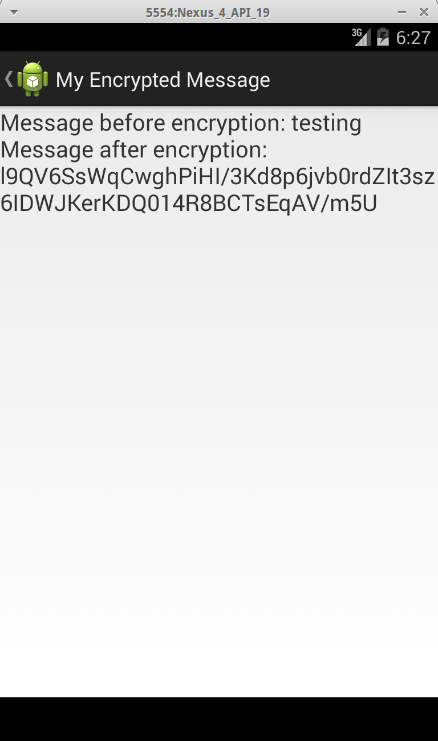
\includegraphics[scale=0.25]{string-encrypting-activity.png}
\caption{String Encryption Activity Screenshot.\label{fig:stringactivity}}
\end{figure}
\subsubsection{Fibonacci Calculator Activity}
The Fibonacci calculator activity takes input from the main activity as an integer and calculated the Fibonacci number up to the given number. Two versions of the Fibonacci Calculator were written. One that correctly handled very large numbers, and one that did not, which causes integer overflow, see Figure \ref{fig:fibo}. The Java code is located in Appendix \ref{app:camathsactivity} and the activity XML is located in Appendix \ref{app:camathsxml}.
\begin{figure}[H]
\begin{subfigure}{0.25\textwidth}
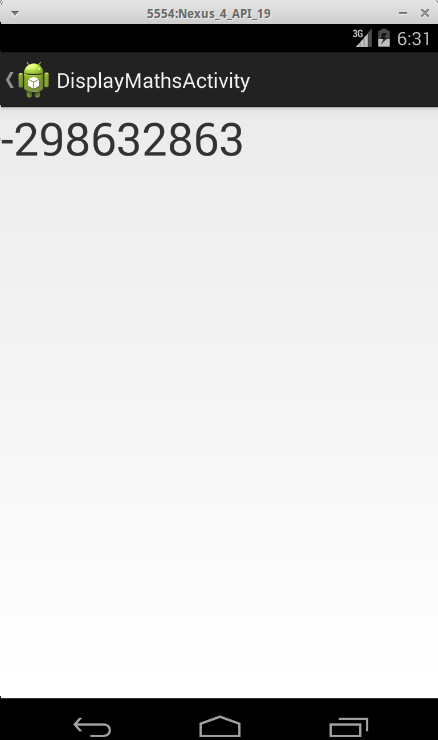
\includegraphics[scale=0.25]{fib-with-overflow-activity.png}
\caption{With Overflow.}
\end{subfigure}%
\begin{subfigure}{0.25\textwidth}
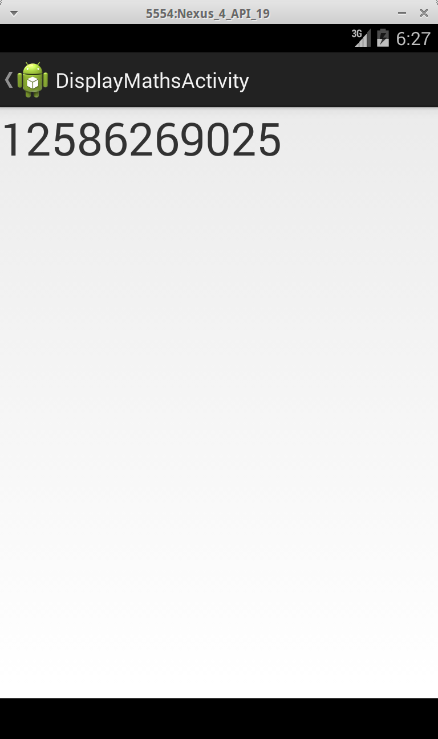
\includegraphics[scale=0.25]{fibo-no-overflow-activity.png}
\caption{Without Overflow.}
\end{subfigure}
\caption{Fibonacci Calculator with and without Overflow Activity Screenshot.\label{fig:fibo}}
\end{figure}
\subsubsection{Web Page Activity}
The web page activity used input from the main activity in the form of a URL and displayed the associated web page. This activity was not fully implemented. It was able to make a connection to the specified URL, but it is not able to render the web page correctly. Having full functionality here is not important. The main point of this activity was to implement network activity and not to properly displaying web pages. This activity can be seen in Figure \ref{fig:webactivity}. The Java code is located in Appendix \ref{app:cawebactivity} and the activity XML is located in Appendix \ref{app:cawebxml}.
\begin{figure}[!ht]
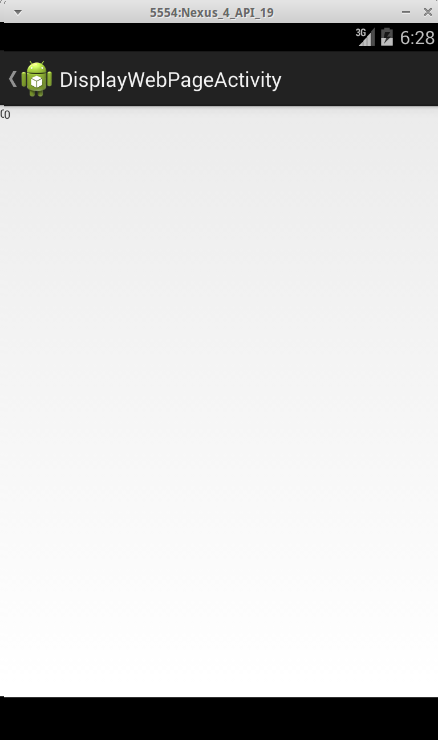
\includegraphics[scale=0.25]{web-activity.png}
\caption{Web Page Activity Screenshot.\label{fig:webactivity}}
\end{figure}
\subsection{Apache Ant Build Process}
Every application was built in release mode, digitally signed, and byte aligned. Release mode directs the build script to build the Android application so that it is ready for distribution to the end-users. This mode removes some information from the resulting APK and requires that it be signed with a keystore. Therefore, a signed key was generated and included along with each application. After the application had been signed it was properly byte aligned, meaning the APK archive was aligned to ensure that all uncompressed data started with a particular alignment relative to the start of the file. This allowed for the best compression rates as well as efficient and proper use of the APK’s.
\subsection{Proguard Obfuscation}
Since Proguard is the default obfuscator released with the Android SDK, enabling Proguard was a simple task. Most of the Proguard settings enabled by default were acceptable to use when obfuscating. However the following settings were enabled to ensure strict obfuscation settings. For a full list of the settings Proguard used, see Appendices \ref{app:opp} and \ref{app:opa}.
\begin{description}
\item[overloadagressivly] \hfill \\ The overloadagressivly setting allows for multiple fields and or methods to use the same name. Any variable in one class could be named the same as a variable in a different class.
\item[flattenpackagehierachy] \hfill \\ The flattenpackagehierachy setting will repackage all the generated or included packages into a single parent APK package.
\end{description}
\subsection{Java Archive Grinder Obfuscation}
The Java Archive Grinder did not function properly as an Ant Task, therefore the resulting obfuscation had to occur after the APK was generated. This task was accomplished by opening the APK archive and finding the Dalvik bytecode, the classes.dex file. The classes.dex file was then converted to Java bytecode using the tool dex2jar. Once the Dalvik bytecode is converted, Java Archive Grinder could then be used. The Java Archive Grinder was set to obfuscate as strictly as possible. Once the obfuscator completed its task, it was converted back into the Dalvik bytecode, using the tool jar2dex, and repackaged into the original APK, replacing the old classes.dex with the obfuscated version.

When attempting to get the Java Archive Grinder to obfuscate as strict as possible it would fail. Java Archive Grinder was failing when attempting bytecode obfuscation. Therefore, the obfuscator was run with the -nobco or no bytecode obfuscation setting. This failure was possibly due to a conversion issue, when it was converted from dexcode to Java bytecode. It may not have correctly converted some of the bytecode. Alternatively, it may have been a problem with the version of the Java bytecode. The Java Archive Grinder obfuscator may have been written using an older version of Java, and could not understand some of the newer bytecode instructions.
\subsection{Zelix KlassMaster Obfuscation}
The Zelix KlassMaster obfuscator was compatible with the Ant build system. The easiest method of using KlassMaster was to replace the call to the Proguard program, with a call to the KlassMaster program. This would force Ant to use KlassMaster instead of Proguard when obfuscation was enabled. KlassMaster functioned by reading in a script file that has the obfuscation settings defined for the Android application. This settings file was generated with a tool that was provided along with KlassMaster that took the Proguard settings and generated an appropriate script file that KlassMaster could understand. After the script file was generated, additional settings were applied to make the obfuscation as strict as possible. The full script is located in Appendix \ref{app:oz}. The following settings were included into the script.
\begin{description}
\item[obfuscateFlow] \hfill \\ The obfuscateFlow setting will make slight changes to the bytecode that will obscure the control flow without changing the code functionality at run time.
\item[exceptionObfuscation] \hfill \\ The exceptionObfuscation setting is similar to the obfuscateFlow setting. It changes the exception handling of the bytecode.
\item[encryptStringLiterals] \hfill \\ The encryptStringLiterals setting encrypts all strings found in the bytecode constant pools. It adds code to the bytecode that will decrypt the strings at run time.
\item[mixedCaseClassNames] \hfill \\ The mixedCaseClassNames setting allows for any class to be named with a random set of characters of any case, upper or lower.
\item[agressiveMethodRenaming] \hfill \\ The agressiveMethodRenaming setting allows for multiple identifiers to be renamed with the same name.
\end{description}
\subsection{Allatori Obfuscation}
Allatori worked with Ant by using an Ant Task. The Ant Task replaced the obfuscation call that would have executed the Proguard obfuscation, but instead executed the Allatori obfuscation. Therefore when running Ant it executed Allatori when the obfuscation step was processed. Allatori runs with a script that defined the settings for obfuscation. The full script is located in Appendix \ref{app:oa}. The script was changed to make the obfuscation as strict as possible. The following settings were added to the base script.
\begin{description}
\item[string encryption] \hfill \\ This setting found all string data and encoded it, and also added in code to allow for the decryption of strings at run time.
\item[control flow obfuscation] \hfill \\ This setting changed the standard Java constructions (loops, conditional, and branching instructions) where possible, and altered the commands such that decompilation is more difficult.
\item[line number obfuscation] \hfill \\ This setting changed any of the line numbers.
\item[remove toString] \hfill \\ This setting removed any call to the toString bytecode instruction.
\end{description}
\end{obeylines}